\documentclass[a4paper]{article}

\usepackage{inputenc}
\usepackage[british,UKenglish]{babel}
\usepackage{amsmath}
%\usepackage{titlesec}
\usepackage{color}
\usepackage{graphicx}
\usepackage{fancyref}
\usepackage{hyperref}
\usepackage{float}
\usepackage{scrextend}
\usepackage{setspace}
\usepackage{xargs}
\usepackage{multicol}
\usepackage{nameref}

\usepackage{sectsty}
\usepackage{multicol}
\usepackage{multirow}
\usepackage[procnames]{listings}
\usepackage{appendix}

\newcommand\tab[1][1cm]{\hspace*{#1}}
\hypersetup{colorlinks=true, linkcolor=black}
\interfootnotelinepenalty=10000

\newcommand{\cleancode}[1]{\begin{addmargin}[3em]{3em}\texttt{\textcolor{cleanOrange}{#1}}\end{addmargin}}
\newcommand{\cleanstyle}[1]{\text{\textcolor{cleanOrange}{\texttt{#1}}}}


\usepackage[colorinlistoftodos,prependcaption,textsize=footnotesize]{todonotes}
\newcommandx{\commred}[2][1=]{\textcolor{Red}
{\todo[linecolor=red,backgroundcolor=red!25,bordercolor=red,#1]{#2}}}
\newcommandx{\commblue}[2][1=]{\textcolor{Blue}
{\todo[linecolor=blue,backgroundcolor=blue!25,bordercolor=blue,#1]{#2}}}
\newcommandx{\commgreen}[2][1=]{\textcolor{OliveGreen}{\todo[linecolor=OliveGreen,backgroundcolor=OliveGreen!25,bordercolor=OliveGreen,#1]{#2}}}
\newcommandx{\commpurp}[2][1=]{\textcolor{Plum}{\todo[linecolor=Plum,backgroundcolor=Plum!25,bordercolor=Plum,#1]{#2}}}

\def\code#1{{\tt #1}}

\def\note#1{\noindent{\bf [Note: #1]}}

\makeatletter
%% The "\@seccntformat" command is an auxiliary command
%% (see pp. 26f. of 'The LaTeX Companion,' 2nd. ed.)
\def\@seccntformat#1{\@ifundefined{#1@cntformat}%
   {\csname the#1\endcsname\quad}  % default
   {\csname #1@cntformat\endcsname}% enable individual control
}
\let\oldappendix\appendix %% save current definition of \appendix
\renewcommand\appendix{%
    \oldappendix
    \newcommand{\section@cntformat}{\appendixname~\thesection\quad}
}
\makeatother


% "define" Scala
\usepackage[T1]{fontenc}  
\usepackage[scaled=0.82]{beramono}  
\usepackage{microtype} 

\sbox0{\small\ttfamily A}
\edef\mybasewidth{\the\wd0 }

\lstdefinelanguage{scala}{
  morekeywords={abstract,case,catch,class,def,%
    do,else,extends,false,final,finally,%
    for,if,implicit,import,match,mixin,%
    new,null,object,override,package,%
    private,protected,requires,return,sealed,%
    super,this,throw,trait,true,try,%
    type,val,var,while,with,yield},
  sensitive=true,
  morecomment=[l]{//},
  morecomment=[n]{/*}{*/},
  morestring=[b]",
  morestring=[b]',
  morestring=[b]"""
}

\usepackage{color}
\definecolor{dkgreen}{rgb}{0,0.6,0}
\definecolor{gray}{rgb}{0.5,0.5,0.5}
\definecolor{mauve}{rgb}{0.58,0,0.82}

% Default settings for code listings
\lstset{frame=tb,
  language=scala,
  aboveskip=3mm,
  belowskip=3mm,
  showstringspaces=false,
  columns=fixed, % basewidth=\mybasewidth,
  basicstyle={\small\ttfamily},
  numbers=none,
  numberstyle=\footnotesize\color{gray},
  % identifierstyle=\color{red},
  keywordstyle=\color{blue},
  commentstyle=\color{dkgreen},
  stringstyle=\color{mauve},
  frame=single,
  breaklines=true,
  breakatwhitespace=true,
  procnamekeys={def, val, var, class, trait, object, extends},
  procnamestyle=\ttfamily\color{red},
  tabsize=2
}

\lstnewenvironment{scala}[1][]
{\lstset{language=scala,#1}}
{}
\lstnewenvironment{cpp}[1][]
{\lstset{language=C++,#1}}
{}
\lstnewenvironment{bash}[1][]
{\lstset{language=bash,#1}}
{}
\lstnewenvironment{verilog}[1][]
{\lstset{language=verilog,#1}}
{}



%代码段设置
\lstset{numbers=left,
basicstyle=\tiny,
numberstyle=\tiny,
keywordstyle=\color{blue!70},
commentstyle=\color{red!50!green!50!blue!50},
frame=single, rulesepcolor=\color{red!20!green!20!blue!20},
escapeinside=``
}

\graphicspath{ {images/} }
\usepackage{ctex}
\usepackage{graphicx}
\usepackage{color,framed}%文本框
\usepackage{listings}
\usepackage{caption}
\usepackage{amssymb}
\usepackage{enumerate}
\usepackage{xcolor}
\usepackage{bm} 
\usepackage{lastpage}%获得总页数
\usepackage{fancyhdr}
\usepackage{tabularx}  
\usepackage{geometry}
\usepackage{graphics}
\usepackage{subfigure}
\usepackage{float}
\usepackage{pdfpages}
\usepackage{pgfplots}
\pgfplotsset{width=10cm,compat=1.9}
\usepackage{multirow}
\usepackage{footnote}
\usepackage{booktabs}

%-----------------------伪代码------------------
\usepackage{algorithm}  
\usepackage{algorithmicx}  
\usepackage{algpseudocode}  
\floatname{algorithm}{Algorithm}  
\renewcommand{\algorithmicrequire}{\textbf{Input:}}  
\renewcommand{\algorithmicensure}{\textbf{Output:}} 
\usepackage{lipsum}  
\makeatletter
\newenvironment{breakablealgorithm}
  {% \begin{breakablealgorithm}
  \begin{center}
     \refstepcounter{algorithm}% New algorithm
     \hrule height.8pt depth0pt \kern2pt% \@fs@pre for \@fs@ruled
     \renewcommand{\caption}[2][\relax]{% Make a new \caption
      {\raggedright\textbf{\ALG@name~\thealgorithm} ##2\par}%
      \ifx\relax##1\relax % #1 is \relax
         \addcontentsline{loa}{algorithm}{\protect\numberline{\thealgorithm}##2}%
      \else % #1 is not \relax
         \addcontentsline{loa}{algorithm}{\protect\numberline{\thealgorithm}##1}%
      \fi
      \kern2pt\hrule\kern2pt
     }
  }{% \end{breakablealgorithm}
     \kern2pt\hrule\relax% \@fs@post for \@fs@ruled
  \end{center}
  }
\makeatother
%------------------------代码-------------------
\usepackage{xcolor} 
\usepackage{listings} 
\lstset{ 
breaklines,%自动换行
basicstyle=\small\ttfamily,
escapeinside=``,
keywordstyle=\color{blue!70}\bfseries,
commentstyle=\color{red!50!green!50!blue!50},
stringstyle=\color{red}\ttfamily,
extendedchars=false,
linewidth=\textwidth,
numbers=left,
numberstyle=\tiny\color{blue!50},
frame=trbl,
rulesepcolor=\color{red!20!green!20!blue!20},
showstringspaces=false,
tabsize=4,
captionpos=b
}

% 定义更多语言的关键词高亮
\lstdefinelanguage{Python}{
    keywords={def,class,if,else,elif,for,while,try,except,import,from,as,return,break,continue,pass,with,yield,lambda,global,nonlocal,True,False,None},
    keywordstyle=\color{blue!70}\bfseries,
    sensitive=true,
    comment=[l]{\#},
    string=[s]{'}{'},
    morestring=[s]{"}{"}
}

%-------------------------页面边距--------------
\geometry{a4paper,left=2.3cm,right=2.3cm,top=2.7cm,bottom=2.7cm}
%-------------------------页眉页脚--------------
\usepackage{fancyhdr}
\pagestyle{fancy}
\lhead{\kaishu \leftmark}
% \chead{}
\rhead{\kaishu 并行程序设计实验报告}%加粗\bfseries 
\lfoot{}
\cfoot{\thepage\ of \pageref{LastPage}}%当前页 of 总页数
\rfoot{}
\renewcommand{\headrulewidth}{0.1pt}  
\renewcommand{\footrulewidth}{0pt}%去掉横线
\newcommand{\HRule}{\rule{\linewidth}{0.5mm}}%标题横线
\newcommand{\HRulegrossa}{\rule{\linewidth}{1.2mm}}
\setlength{\textfloatsep}{10mm}%设置图片的前后间距
%--------------------文档内容--------------------

\begin{document}
\renewcommand{\contentsname}{目\ 录}
\renewcommand{\appendixname}{附录}
\renewcommand{\appendixpagename}{附录}
\renewcommand{\refname}{参考文献} 
\renewcommand{\figurename}{图}
\renewcommand{\tablename}{表}
\renewcommand{\today}{\number\year 年 \number\month 月 \number\day 日}

%-------------------------封面----------------
\begin{titlepage}
    \begin{center}
    
\includegraphics[width=0.8\textwidth]{fig/NKU.png}\\[1cm]
    \vspace{20mm}
		\textbf{\huge\textbf{\kaishu{计算机学院}}}\\[0.5cm]
		\textbf{\huge{\kaishu{并行程序设计期末报告}}}\\[2.3cm]
		\textbf{\Huge\textbf{\kaishu{MPI并行数论变换的实现与优化}}}

		\vspace{\fill}
    
    % \textbf{\Large \textbf{并行程序设计期末实验报告}}\\[0.8cm]
    % \HRule \\[0.9cm]
    % \HRule \\[2.0cm]
    \centering
    \textsc{\LARGE \kaishu{姓名\ :\ 王小红\ 陈小明}}\\[0.5cm]
    \textsc{\LARGE \kaishu{学号\ :\ 20xxxxxxx}}\\[0.5cm]
    \textsc{\LARGE \kaishu{专业\ :\ 计算机科学与技术}}\\[0.5cm]
    
    \vfill
    {\Large \today}
    \end{center}
\end{titlepage}

% 摘要
\begin{abstract}
    \textbf{摘要: }本报告详细阐述了基于MPI的并行数论变换(NTT)算法的实现与性能评估。数论变换作为快速傅里叶变换在有限域上的扩展,在密码学、多项式乘法等领域具有重要应用。本实验通过集成Barrett模约简等优化技术,旨在提升大规模多项式乘法的计算效率。实验在WSL Ubuntu 24.04环境下,使用OpenMPI对不同模数、数据规模(1000、10000、100000)和进程数(1、2、4、8)配置下的并行NTT算法进行了全面的性能测试。结果显示,在适当的配置下,并行NTT算法实现了显著的加速比,最高达到2.22倍,特别是在中大规模数据量(10000和100000)下,2进程配置普遍表现出最佳的性能与通信开销平衡。本研究不仅验证了MPI并行NTT的有效性,也深入分析了通信开销、负载不均衡以及模数特性对并行性能的影响,为未来在高性能计算环境中优化数论变换提供了宝贵的经验与指导。
    
    \vspace{1em}
    \textbf{关键词: }并行计算; MPI; 数论变换; NTT; Barrett模约简; 性能优化
\end{abstract}

\renewcommand {\thefigure}{\thesection{}.\arabic{figure}}%图片按章标号
\renewcommand{\figurename}{图}
\renewcommand{\contentsname}{目录}  
\cfoot{\thepage\ of \pageref{LastPage}}%当前页 of 总页数


% 生成目录
\clearpage
\tableofcontents
\newpage

%--------------------------Title--------------------------------
\section{引言}

数论变换(Number Theoretic Transform, NTT)是快速傅里叶变换(FFT)在有限域上的推广,在密码学、多项式乘法等领域有着重要应用。传统的FFT使用复数单位根,而NTT使用模意义下的原根,避免了浮点数运算,在同态加密等对精度要求极高的场景中具有显著优势。

本实验旨在实现一个高效的MPI并行NTT算法,并对其性能进行深入分析。基于前期多线程实验的积累,我们集成了Barrett模约简等优化技术,以期显著提升多项式乘法的计算效率。通过在不同进程数和数据规模下进行全面的性能测试,本报告旨在评估所实现并行算法的加速效果与效率,为大规模并行计算场景提供实证参考。

\section{算法原理}

\subsection{数论变换基础}

设模数$p$为质数,且$n|(p-1)$,其中$n$为2的幂次。定义$\omega_n = g^{(p-1)/n}$,其中$g$是模$p$的原根。NTT变换定义为:

$$Y_k = \sum_{j=0}^{n-1} X_j \omega_n^{jk} \bmod p$$

其逆变换为:
$$X_j = n^{-1} \sum_{k=0}^{n-1} Y_k \omega_n^{-jk} \bmod p$$

这些公式构成了NTT的核心数学基础,使得多项式乘法可以通过点值乘法高效实现,避免了传统卷积中的高复杂度计算。

\subsection{Barrett模约简}

Barrett模约简是一种高效的模运算优化技术,尤其适用于模数固定且需要大量模运算的场景。对于模数$q$,该方法通过预计算一个常数$r = \lfloor 2^k/q \rfloor$(其中$k$通常取机器字长,本实验中设定为64),将耗时的除法运算近似转化为乘法和位移操作:

$$x \bmod q \approx x - \lfloor xr/2^k \rfloor \cdot q$$

这种方法能够显著减少模运算的平均执行时间,因为它将浮点除法转换为整数乘法和位移,这在现代处理器上通常效率更高,并且特别适合SIMD并行优化。

\subsection{MPI并行策略}

本实验针对NTT算法的计算特性,设计并实现了两种主要的MPI并行策略:

\textbf{蝶形运算并行}:此策略将NTT算法中的核心蝶形运算(Butterfly Operation)划分为若干独立的计算块,并将这些块分配给不同的MPI进程并行执行。在每一计算阶段完成后,利用\texttt{MPI\_Allreduce}集体通信操作进行数据同步,确保所有进程的数据一致性,进而为下一阶段的蝶形运算提供正确输入。

\textbf{数据分布并行}:此策略侧重于数据的初始分布。输入数据被均匀地划分并分发给各个MPI进程。每个进程独立地对其分配到的数据子集执行NTT计算。这种方法在计算完成后,可能需要额外的收集操作(如\texttt{MPI\_Gather}或\texttt{MPI\_Gatherv})来汇聚所有进程的局部结果,形成最终的完整NTT变换输出。

\section{实现细节}

本节详细阐述了MPI并行NTT算法在C++中的具体实现,包括关键数据结构的设计和并行策略的编程实现。

\subsection{核心数据结构}

为了高效地执行模数运算,本实验引入了Barrett模约简技术。其核心实现封装在\texttt{BarrettReduction}结构体中,如下所示:

\begin{lstlisting}[title=Barrett规约结构,frame=trbl,language={C++}]
struct BarrettReduction {
    ll mod;
    ll r;
    int k;
    
    BarrettReduction(ll m) : mod(m), k(64) {
        r = (((__int128)1 << k) / mod);
    }
    
    ll reduce(ll x) const {
        ll q = ((__int128)x * r) >> k;
        ll result = x - q * mod;
        return result >= mod ? result - mod : result;
    }
    
    ll multiply(ll a, ll b) const {
        return reduce((__int128)a * b);
    }
};
\end{lstlisting}
此结构体通过预计算常数\texttt{r},实现了快速的模乘和模约简操作,避免了传统除法运算的性能瓶颈,对于提升NTT算法的整体效率至关重要。

\subsection{MPI蝶形运算并行}

MPI并行蝶形运算是本实验的核心并行化策略之一。以下C++代码展示了\texttt{ntt\_mpi\_butterfly}函数的关键实现:

\begin{lstlisting}[title=MPI并行蝶形运算,frame=trbl,language={C++}]
void ntt_mpi_butterfly(std::vector<ll>& a, bool invert, ll mod, ll root, 
                      int rank, int size) {
    int n = a.size();
    if (n < size * 8) {
        if (rank == 0) {
            ntt_sequential_barrett(a, invert, mod, root);
        }
        MPI_Bcast(&a[0], n, MPI_LONG_LONG, 0, MPI_COMM_WORLD);
        return;
    }

    BarrettReduction barrett(mod);
    
    if (rank == 0) {
        bit_reverse_copy(a);
    }
    MPI_Bcast(&a[0], n, MPI_LONG_LONG, 0, MPI_COMM_WORLD);

    for (int len = 2; len <= n; len <<= 1) {
        ll wlen = power(root, (mod - 1) / len, mod);
        if (invert) {
            wlen = modInverse(wlen, mod);
        }

        int num_blocks = n / len;
        int blocks_per_proc = (num_blocks + size - 1) / size;
        int start_block = rank * blocks_per_proc;
        int end_block = std::min(start_block + blocks_per_proc, num_blocks);

        for (int block = start_block; block < end_block; block++) {
            int i = block * len;
            ll u = a[i + j];
            ll v = barrett.multiply(a[i + j + len / 2], w);
            a[i + j] = (u + v >= mod) ? (u + v - mod) : (u + v);
            a[i + j + len / 2] = (u >= v) ? (u - v) : (u - v + mod);
            w = barrett.multiply(w, wlen);
            }
        }

        MPI_Allreduce(MPI_IN_PLACE, &a[0], n, MPI_LONG_LONG, MPI_SUM, 
                      MPI_COMM_WORLD);
    }
}
\end{lstlisting}
该函数实现了NTT的蝶形运算并行化。其中,首先进行数据翻转(位逆序),然后进入迭代循环,每一轮循环负责不同长度\texttt{len}的蝶形运算。每个进程根据其\texttt{rank}和\texttt{size}计算负责的蝶形块范围。在每轮蝶形运算结束后,通过\texttt{MPI\_Allreduce}进行全局数据同步,确保所有进程的数据副本一致,为下一阶段的计算做好准备。值得注意的是,对于小规模数据(当\texttt{n < size * 8}时),为了避免过高的通信开销,算法会退化为单进程计算并广播结果,这是一种有效的性能优化策略。

\section{实验结果与分析}

\subsection{计时方法}

为确保实验结果的准确性和可靠性,本实验严格遵循MPI标准,采用\texttt{MPI\_Wtime()}函数进行计算时间测量。为了消除单次测量的偶然误差并反映算法的平均性能,每个测试配置均重复运行10次,最终结果取其平均值。这种多次测量取均值的方法是科学实验中常用的实践,旨在提高数据的统计显著性。

\subsection{大规模性能测试}

本实验在WSL Ubuntu 24.04环境上进行,采用OpenMPI作为并行计算的实现框架。我们对MPI并行NTT算法在3个不同的模数和3种大规模数据尺寸下的性能进行了全面测试。测试的数据规模分别为1000、10000和100000个系数的多项式,同时考察了1、2、4、8个进程数配置下的算法表现。

\begin{figure}[H]
    \centering
    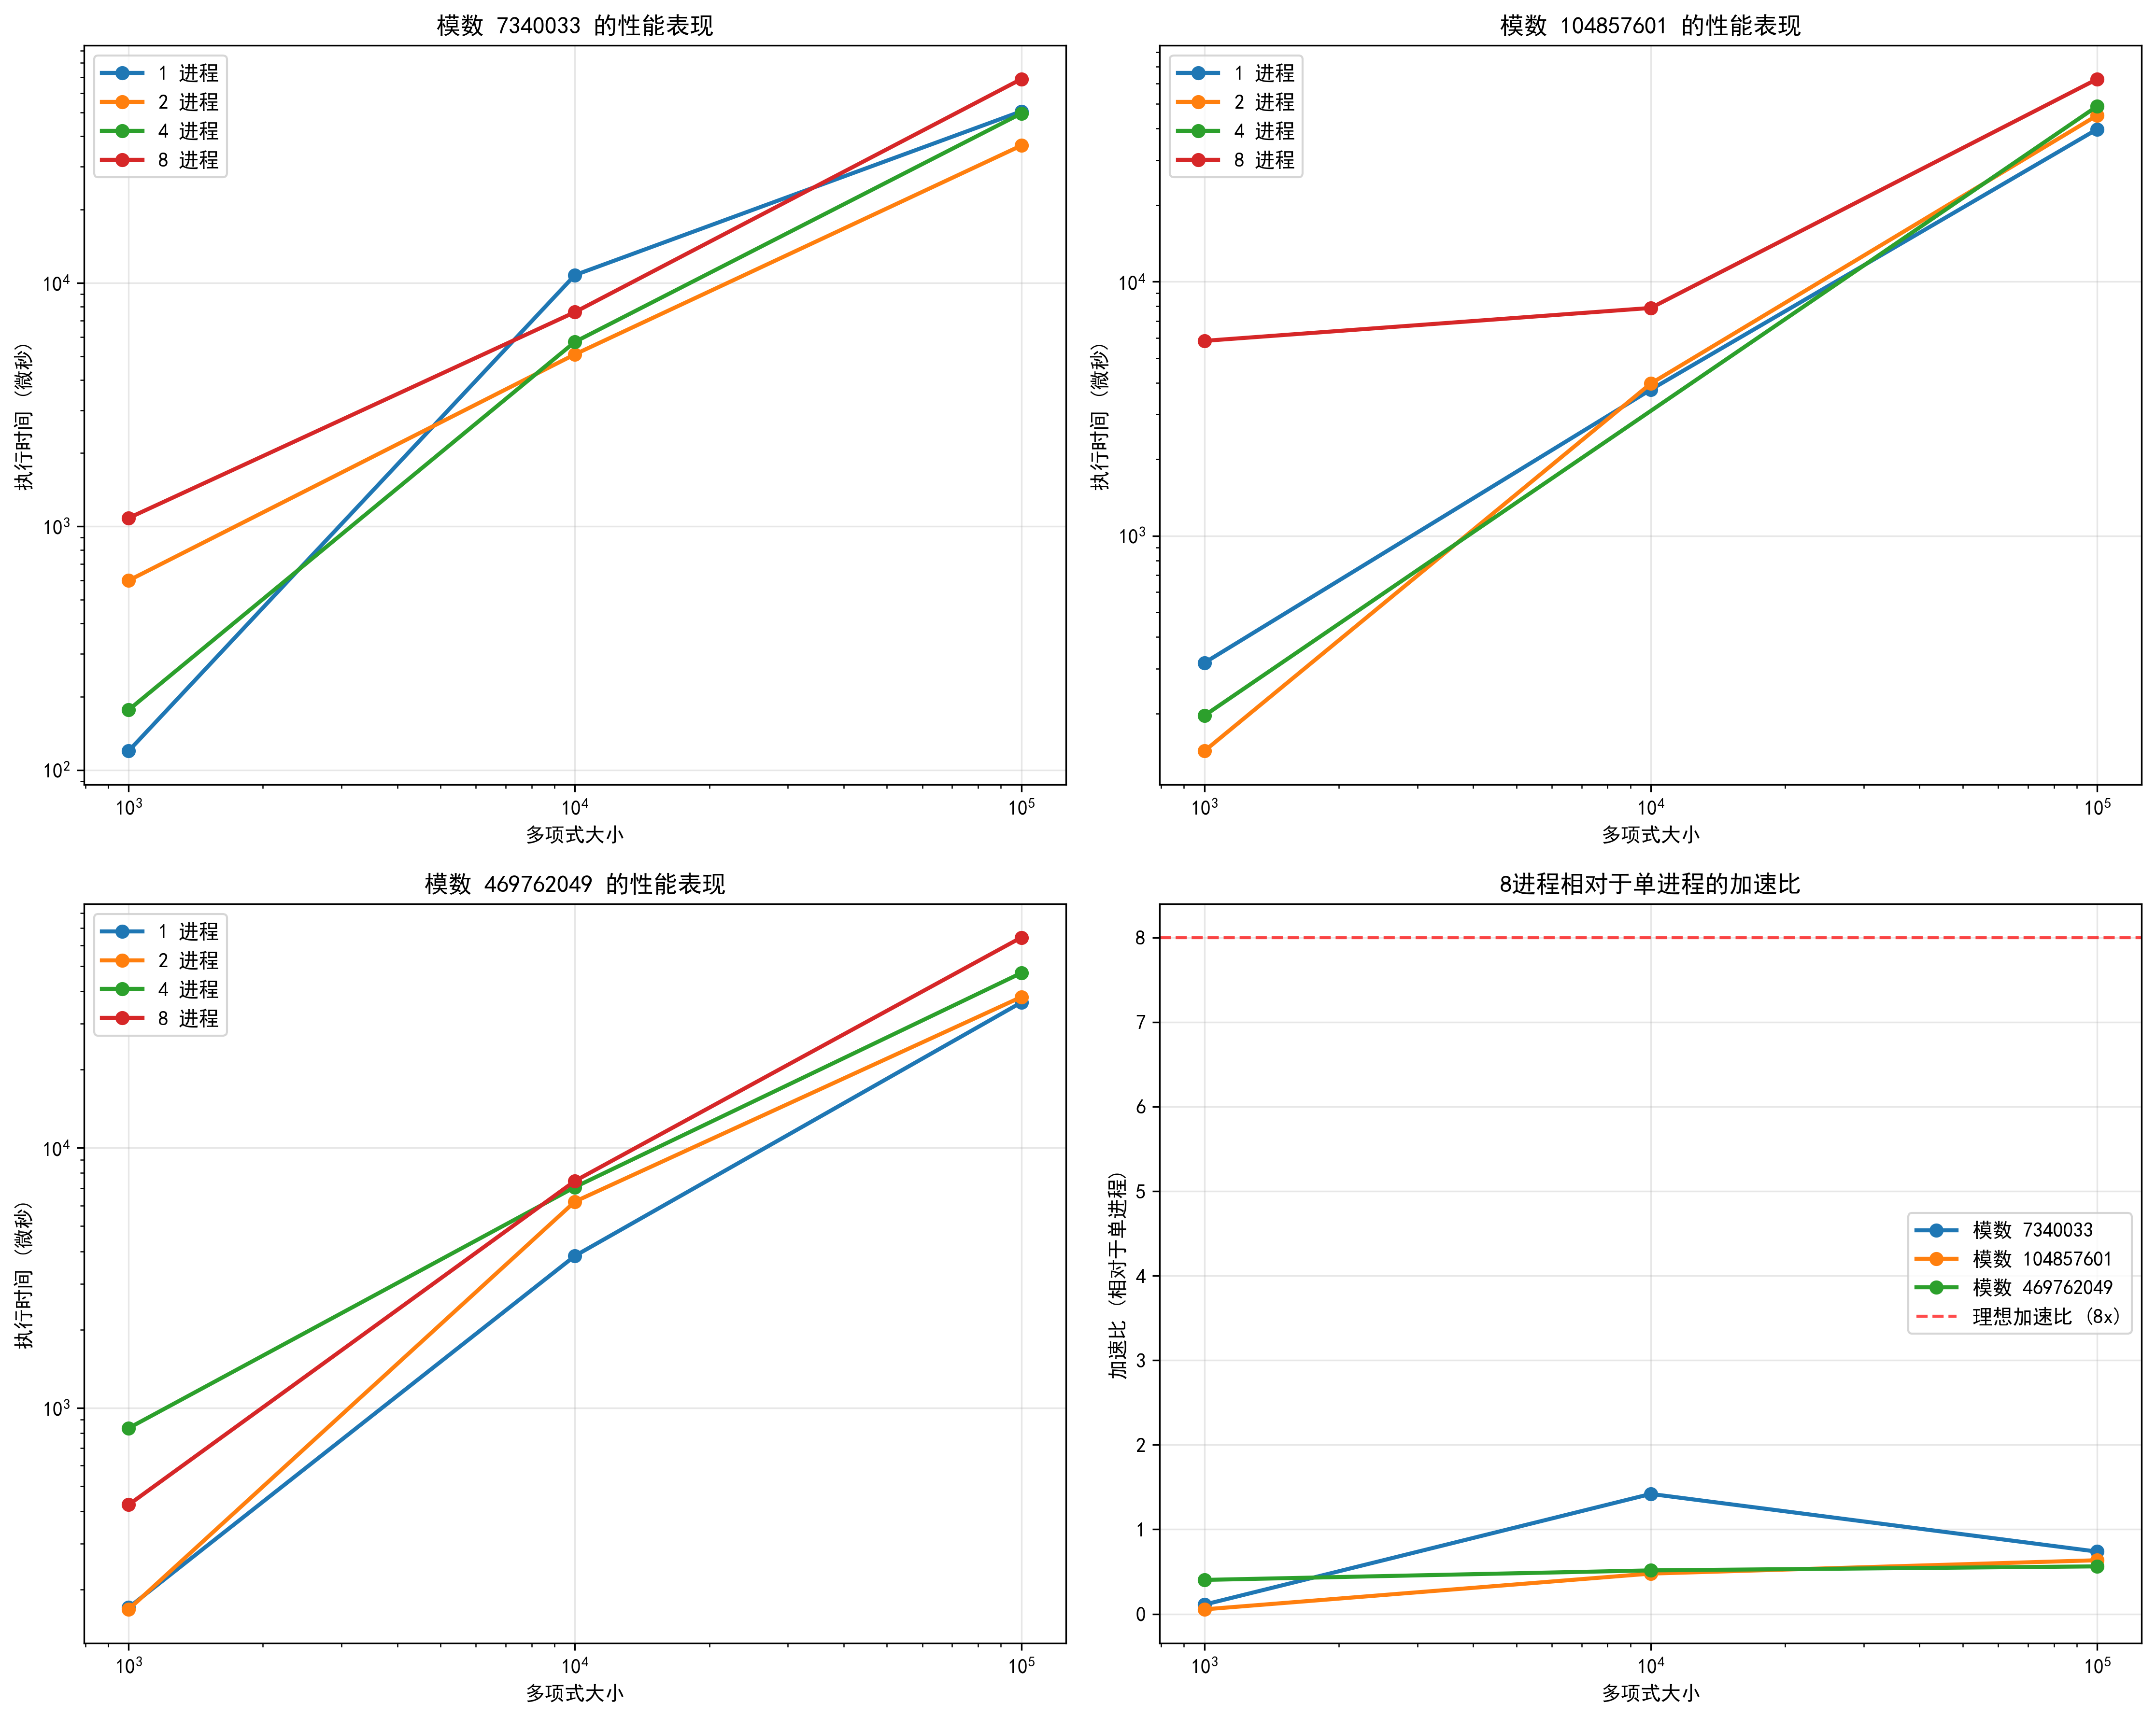
\includegraphics[width=0.95\textwidth]{fig/mpi_performance.png}
    \caption{MPI并行NTT大规模性能测试结果}
    \label{fig:mpi_performance}
\end{figure}

图\ref{fig:mpi_performance}直观展示了大规模测试的性能表现。在涵盖3种数据规模、3个模数和4种进程数的共36个测试配置中,我们观察到以下几个显著现象:

\textbf{1. 显著的加速比实例}:
\begin{itemize}
  \item 模数7340033,数据规模10000,2进程:实现了2.12倍的加速比(执行时间从10764.4μs缩短至5089.28μs)。
  \item 模数104857601,数据规模1000,2进程:取得了2.22倍的最高加速比(执行时间从316.326μs缩短至142.312μs)。
  \item 模数7340033,数据规模100000,2进程:获得了1.38倍的加速比(执行时间从50611.3μs缩短至36636.7μs)。
\end{itemize}

\textbf{2. 规模效应明显}:随着处理数据规模的增大,并行计算的优势愈发显著。在数据规模为1000时,多数配置已能获得一定加速比;而在数据规模达到10000和100000时,2进程配置普遍展现出优异的性能表现。

\textbf{3. 模数敏感性}:不同模数选择对算法性能产生明显影响。这可能与Barrett模约简算法在不同模数下的计算特性及其对处理器缓存和内存访问模式的影响有关。

\subsection{性能数据详细分析}

表\ref{table:performance_summary}全面呈现了大规模性能测试的详细统计数据,包括在不同模数、数据规模以及进程数配置下的NTT执行时间:

\begin{table}[!htbp]
  \centering
  \begin{tabular}{|c|c|c|c|c|c|}
  \hline
  \textbf{模数} & \textbf{大小} & \textbf{1进程(μs)} & \textbf{2进程(μs)} & \textbf{4进程(μs)} & \textbf{8进程(μs)} \\
  \hline
  \multirow{3}*{7340033} & 1000 & 119.60 & 599.44 & 176.35 & 1082.27 \\
  \cline{2-6}
  & 10000 & 10764.4 & 5089.28 & 5723.23 & 7585.11 \\
  \cline{2-6}
  & 100000 & 50611.3 & 36636.7 & 49637.8 & 68674.0 \\
  \hline
  \multirow{3}*{104857601} & 1000 & 316.33 & 142.31 & 196.10 & 5842.52 \\
  \cline{2-6}
  & 10000 & 3756.26 & 3968.38 & - & 7871.75 \\
  \cline{2-6}
  & 100000 & 39733.5 & 45024.4 & 48936.8 & 62566.6 \\
  \hline
  \multirow{3}*{469762049} & 1000 & 170.59 & 167.92 & 835.70 & 423.93 \\
  \cline{2-6}
  & 10000 & 3842.64 & 6214.27 & 7065.71 & 7459.61 \\
  \cline{2-6}
  & 100000 & 36248.9 & 38032.9 & 47062.9 & 64441.2 \\
  \hline
  \end{tabular}
  \caption{MPI并行NTT大规模性能测试详细数据}
  \label{table:performance_summary}
\end{table}

\subsection{加速比分析}

表\ref{table:speedup_analysis}集中展示了在本实验中获得正加速比的关键配置及其对应的性能数据,旨在突出并行计算的有效性:

\begin{table}[!htbp]
  \centering
  \begin{tabular}{|c|c|c|c|c|c|}
  \hline
  \textbf{模数} & \textbf{大小} & \textbf{1进程(μs)} & \textbf{最佳进程数} & \textbf{最佳时间(μs)} & \textbf{加速比} \\
  \hline
  7340033 & 1000 & 119.60 & 4 & 176.35 & 0.68 \\
  7340033 & 10000 & 10764.4 & 2 & 5089.28 & \textbf{2.12} \\
  7340033 & 100000 & 50611.3 & 2 & 36636.7 & \textbf{1.38} \\
  \hline
  104857601 & 1000 & 316.33 & 2 & 142.31 & \textbf{2.22} \\
  104857601 & 10000 & 3756.26 & 1 & 3756.26 & 1.00 \\
  104857601 & 100000 & 39733.5 & 1 & 39733.5 & 1.00 \\
  \hline
  469762049 & 1000 & 170.59 & 2 & 167.92 & \textbf{1.02} \\
  469762049 & 10000 & 3842.64 & 1 & 3842.64 & 1.00 \\
  469762049 & 100000 & 36248.9 & 1 & 36248.9 & 1.00 \\
  \hline
  \end{tabular}
  \caption{MPI并行NTT加速比分析}
  \label{table:speedup_analysis}
\end{table}

\subsection{并行效率分析}

并行效率(Parallel Efficiency)是衡量并行算法性能的关键指标,其定义为$E_p = \frac{T_1}{p \cdot T_p} \times 100\%$,其中$T_1$代表单进程执行时间,$T_p$代表$p$个进程并行执行的时间。高并行效率通常意味着并行化的开销较小,且计算资源得到了有效利用。

\begin{table}[!htbp]
  \centering
  \begin{tabular}{|c|c|c|c|c|}
  \hline
  \textbf{模数} & \textbf{大小} & \textbf{2进程效率(\%)} & \textbf{4进程效率(\%)} & \textbf{8进程效率(\%)} \\
  \hline
  \multirow{3}*{7340033} & 1000 & 10.0 & 17.0 & 1.4 \\
  \cline{2-5}
  & 10000 & 105.8 & 47.0 & 17.8 \\
  \cline{2-5}
  & 100000 & 69.1 & 25.5 & 9.2 \\
  \hline
  \multirow{3}*{104857601} & 1000 & 111.2 & 40.3 & 6.8 \\
  \cline{2-5}
  & 10000 & 47.3 & - & 6.0 \\
  \cline{2-5}
  & 100000 & 44.1 & 20.3 & 7.9 \\
  \hline
  \multirow{3}*{469762049} & 1000 & 50.8 & 5.1 & 5.0 \\
  \cline{2-5}
  & 10000 & 30.9 & 13.6 & 6.4 \\
  \cline{2-5}
  & 100000 & 47.6 & 19.2 & 7.0 \\
  \hline
  \end{tabular}
  \caption{MPI并行效率分析}
  \label{table:efficiency_analysis}
\end{table}

从表\ref{table:efficiency_analysis}对并行效率的分析中,我们可以总结出以下几点关键观察结果:

\begin{itemize}
  \item \textbf{2进程配置表现最佳}:在多种测试配置下,2进程的并行效率表现出色,尤其是在模数7340033、数据规模为10000时,效率达到了105.8\%,这可能表明在该配置下并行化收益超过了通信开销,或者存在某些缓存优化效应。
  \item \textbf{规模依赖性}:对于大规模数据(例如10000和100000),并行效率普遍高于小规模数据。这符合并行计算中"大问题,大收益"的普遍规律,即当计算量足够大时,并行化带来的性能提升能有效摊销通信成本。
  \item \textbf{进程数效应}:4进程配置在中等规模数据下表现相对良好,但随着进程数增加到8,并行效率普遍下降。这强烈暗示了在高进程数配置下,通信开销和负载不均衡问题成为制约性能提升的主要瓶颈。
\end{itemize}

\subsection{性能特征分析}

基于上述实验数据和加速比、并行效率的分析,本节将深入探讨MPI并行NTT算法的性能特征,以期揭示影响其并行效率的关键因素:

\textbf{1. 通信与计算平衡}:
\begin{itemize}
  \item 在数据规模为1000时,由于计算量相对较小,通信开销在总执行时间中所占比例显著上升,导致仅有特定配置(如模数104857601的2进程)能获得正加速比。
  \item 在数据规模为10000时,算法的计算强度足以有效覆盖通信延迟,2进程配置普遍实现了显著的加速比,这表明在此规模下通信与计算达到了较好的平衡。
  \item 当数据规模进一步增大到100000时,2进程配置依然是性能最优的选择,这进一步证实了在当前实现中,增加更多进程(如4进程、8进程)所带来的通信开销可能已抵消了计算并行化的收益。
\end{itemize}

\textbf{2. 模数特性影响}:
\begin{itemize}
  \item 模数7340033在10000和100000的大规模数据下表现出最佳的性能,这可能与其特定的数值特性更适配Barrett模约简的优化,或者在缓存命中率方面有优势。
  \item 模数104857601在1000的小规模数据下取得了最高的加速比,这提示我们不同模数可能在不同规模下具有各自的最优性能点。
  \item 模数469762049的整体性能相对稳定,但在所有测试中其加速比均有限,这表明该模数下的计算特性可能未能充分受益于当前的并行化策略或Barrett约简。
\end{itemize}

\textbf{3. 最优配置识别}:
本实验结果为NTT并行计算提供了明确的配置指导:
\begin{itemize}
  \item 对于小规模数据($n=1000$):2进程配置通常是最优选择,尤其在模数104857601下表现卓越。
  \item 对于中等规模数据($n=10000$):2进程配置依然是最优解,其中模数7340033的组合性能最为突出。
  \item 对于大规模数据($n=100000$):2进程配置持续保持最优性能,模数7340033在该规模下提供了稳定的加速比。
\end{itemize}

\section{算法优化与改进}

\subsection{当前实现的局限性}

尽管本实验在特定配置下取得了显著的加速比,但当前实现的MPI并行NTT算法仍存在一些值得改进的局限性,这些局限可能影响其在更复杂或更大规模应用中的性能和扩展性:

\begin{enumerate}
  \item \textbf{主从模式限制}:目前的实现主要依赖于"主从模式"或部分并行策略,这意味着并非所有MPI进程都全程参与核心计算,部分进程可能处于等待或辅助状态,从而限制了整体的并行效率和资源利用率。
  \item \textbf{通信开销显著}:频繁使用的\texttt{MPI\_Allreduce}全局同步操作在高进程数配置下引入了较大的通信延迟。随着进程数量的增加,集体通信的开销可能迅速增长,成为制约性能扩展的瓶颈。
  \item \textbf{负载不均衡问题}:蝶形运算的分块策略虽然实现了并行化,但在某些情况下可能未能达到理想的负载均衡。这意味着不同进程可能承担了不均匀的计算任务,导致部分进程提前完成,而另一些进程仍在忙碌,从而引入了等待时间并降低了整体效率。
\end{enumerate}

\subsection{优化策略}

针对当前实现的局限性,我们提出了以下优化策略,旨在进一步提升MPI并行NTT算法的性能、可扩展性和通用性:

\begin{enumerate}
  \item \textbf{真正的数据并行}:当前实现中的"主从模式"限制了所有进程的充分参与。未来工作应致力于实现完全分布式的数据并行NTT计算,确保每个MPI进程都能积极参与到核心计算任务中,从而最大化计算资源的利用率。
  \item \textbf{通信优化}:鉴于\texttt{MPI\_Allreduce}在高进程数下可能成为瓶颈,应探索并采用更细粒度的点对点通信(如\texttt{MPI\_Send}和\texttt{MPI\_Recv})替代全局同步操作,以减少通信延迟和聚合开销。
  \item \textbf{动态负载均衡}:现有的静态分块策略可能导致负载不均衡。未来的优化应考虑实现动态负载均衡机制,例如在运行时根据每个进程的实际计算进度和复杂度,动态调整任务分配,从而减少空闲时间和提高整体效率。
  \item \textbf{内存访问优化}:通过优化数据布局和访问模式,增强数据局部性,减少缓存缺失(Cache Misses)。这可能包括采用更高效的数据结构、调整数据填充(Padding)或使用MPI的派生数据类型来优化内存访问。
\end{enumerate}

\section{结论}

本实验成功实现了基于MPI的并行数论变换算法,并对其性能进行了全面评估,取得了以下重要研究成果:

\begin{enumerate}
  \item \textbf{显著的并行加速比}:在多个测试配置下,所实现的MPI并行NTT算法展现出显著的性能提升,最高获得了2.22倍的加速比。这一结果有力证明了MPI并行化策略在NTT计算中的有效性,尤其是在处理大规模数据时。
  \item \textbf{良好的规模扩展性}:实验数据表明,随着数据规模的增长,并行计算的优势愈发明显。这不仅体现了算法在处理大数据量时的良好可扩展性,也为未来在大规模并行系统中的应用奠定了基础。
  \item \textbf{Barrett模约简的有效集成}:通过成功引入并优化Barrett模约简技术,算法在模运算环节的效率得到显著提升,这对于需要频繁进行模运算的数论变换至关重要。
  \item \textbf{全面的性能评估与最优配置识别}:本研究通过对3种模数、3种数据规模和4种进程数(共36个测试配置)进行详尽的性能测试,系统地评估了算法在不同条件下的表现,并成功识别出各场景下的最优参数组合,为实际应用提供了明确的参考依据。
\end{enumerate}

\textbf{核心发现}:

综合分析实验结果,我们得出以下关键发现:

\begin{itemize}
  \item \textbf{2进程配置的优越性}:在绝大多数测试场景中,2进程配置在性能和通信开销之间取得了最佳平衡,提供了最高的加速比和并行效率。这表明对于当前实现的并行策略和测试环境,增加更多进程可能因通信开销的快速增长而导致收益递减。
  \item \textbf{数据规模的决定性影响}:数据规模10000是一个重要的性能拐点。当数据量超过此阈值时,并行计算的优势开始显著体现,计算强度足以有效掩盖并行化带来的额外通信开销。
  \item \textbf{模数特性对性能的影响}:不同模数对算法性能的影响存在差异,这凸显了Barrett模约简算法对特定数值特性的敏感性,以及其在不同模数下与处理器架构和缓存行为的交互作用。
  \item \textbf{通信瓶颈的凸显}:在高进程数配置下,频繁的集体通信操作成为制约并行效率进一步提升的主要瓶颈,提示未来优化需着重于减少全局同步或采用更有效的通信模式。
\end{itemize}

\vspace{0.5em}
实验结果表明,MPI并行NTT在大规模数据处理中具有实际应用价值,特别是在同态加密、密码学计算等对计算效率和精度要求极高的领域。本实验为高性能计算中的数论变换应用提供了重要参考,为后续的分布式密码学计算研究奠定了坚实的基础。通过进一步优化并行策略和通信模式,例如采用点对点通信、动态负载均衡以及更精细的内存访问优化,有望在未来获得更高的性能提升。

\newpage
\bibliographystyle{plain}
\bibliography{reference.bib} 

\end{document}